\section{Circuito N° 1}



\subsection{Esquematico y datos}

Se realiza el análisis teórico del circuito que se muestra en la siguiente figura. 
 

\begin{figure}[h!]
    \centering
    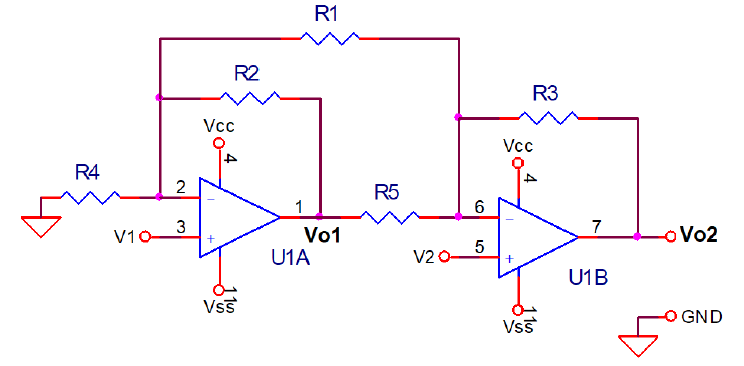
\includegraphics[width=0.80\linewidth]{Secciones/Circuito1/esquematico.png}
    \caption{Esquematico del circuito N° 1}
    \label{fig:esquematico}
\end{figure}

Datos:

\begin{itemize}
  \item Amplificador operacional: LM324
  \item $V_{cc} = 10 \, \text{[V]}$
  \item $V_{ss} = -10 \, \text{[V]}$
  \item $R_1 = R_2 = R_3 = R_4 = R_5 = R$
\end{itemize}

\subsection{Análisis teorico}
Para facilitar el analisis del circuito, consideramos AO ideal, dividimos en 2 casos y luego aplicaremos el teorema de la superposición.

\vspace{1em}

\textbf{Caso 1:} Pasivamos la fuente $V_2$, quedando asi: $V_1 \neq 0 $ y $V_2 = 0$ .

\vspace{1em}

Primero calculamos la ganancia $\frac{V_{O1}}{V_1}$ de la primer etapa. Para esto tengamos en cuenta que $R_1$ y $R_4$ quedan en paralelo. 

\vspace{1em}

\[{R_p = {(R_1 // R_4)} = \frac{R_1 \cdot R_4}{R_1 + R_4}}\]

Luego tenemos que: 

\[I_{R_2} = I_{R_p}\]

\[\frac{V_{01} - V_1}{R_2}
      = \frac{V_1 - 0}{R_p}\]

Si distribuimos y reagrupamos terminos.

\[\frac{V_{01}}{R_2} = \Bigl(\frac{1}{R_p}+\frac{1}{R_2}\Bigl) \cdot {V_1}\]
      
\[{V_{01}} = \Bigl(\frac{R_2}{R_p}+{1}\Bigl) \cdot {V_1}\]

Por lo tanto la primera etapa queda como un no inversor:


\begin{equation}\label{eq:primera_etapa} 
\frac{V_{01}}{V_1} = \frac{R_2}{R_p}+{1}
\end{equation}

      
Ahora calculamos la ganancia $\frac{V_{02}}{V_{01}}$ de la se la segunda etapa:

\[I_{R_3} = I_{R_5}\]


\[\frac{V_{02} - 0 }{R_3} = \frac{0 - V_{01}}{R_5}\]


Despejamos y obtenemos la ganancia de la segunda etapa con respecto a la primera:

\[V_{02} = -(\frac{R_3}{R_5}) \cdot {V_{01}}\]   


\begin{equation}\label{eq:segunda_etapa} 
\frac{V_{02}}{V_{01}} = -\frac{R_3}{R_5}
\end{equation}

Por lo tanto la ganancia para el Caso 1, reemplazando \eqref{eq:primera_etapa} en \eqref{eq:segunda_etapa} tenemos:

\[ A_{V1} = \frac{V_{02}}{V_{01}} \cdot \frac{V_{01}}{V_1} = -\frac{R_3}{R_5} \cdot (\frac{R_2}{R_p}+{1})  \]

\vspace{1em}

\textbf{Caso 2:} Pasivamos la fuente $V_1$, quedando asi: $V_1 = 0$ y $V_2 \neq 0$

\vspace{1em}

Aplicamos la ley de las corrientes en los nodos en la primer etapa:


\[I_{R2} + I_{R1} = 0 \]


\[\frac{V_{01}}{R_2} = -\frac{V_2}{R_1}\]


\[{V_{01}} = -(\frac{R_2}{R_1}) \cdot {V_2}\]

Considerando que lo siguiente:

\[{R_1}={R_2}={R_3}={R_4}={R_5}
      = {R}\]
Entonces, se tiene:
 
 
 \[{V_{01}} = -{V_2}\]
Analizando la segunda etapa se tiene:

\[\frac{V_o-V_2}{R_3}
      = \frac{V_2-V_x}{R_5}+\frac{V_2}{R_1}\]

\begin{equation}\label{eq:condicion} 
\frac{V_o}{R_3} = (\frac{1}{R_5}+\frac{1}{R_1}+\frac{1}{R_1}) \cdot {V_2}-\frac{V_x}{R_5}
\end{equation}
Por la condición \ref{eq:condicion} se tiene
  \[{V_o}=3 \cdot {V_2}+{V_2}\]
      \[{V_o}=4 \cdot {V_2}\]
      
\subsection{Análisis de modo diferencial y en modo común }

Se analiza $V_d$ (diferencial) y $V_c$ (común) teniendo en cuenta que cualquiera de las salidas es una combinación lineal de las tensiones de entrada y las definiciones de las señales en modo común y diferencial dadas.

Primero se tiene:

\[ v_{o\mu}= G_1 v_1 + G_2 v_2\]
y además se tiene:
\[{v_d}
      = {v_2-v_1}\]\[{v_c}
      = \frac{v_1+v_2}{2}\]

Combinando para \(v_1\) y \(v_2\), y sumando miembro a miembro:

\[v_o\mu= (G_1 + G_2)v_1 + G2 v_d \]
\[v_o\mu= (G_1 + G_2)v_2 - G1 v_d \]
\[v_o\mu= \frac{G_1 + G_2}{2}v_c + \frac{G_2-G_1}{2} v_d \]

Por último se tiene:

\[v_{o1}= 2v_c-2_{vd}\]
\[v_{o2}= 4_{vd}\]
\subsection{Impedancias vistas por fuentes de señal }

Como la señal que se inyecta directamente en la entrada de los amplificadores VFA, las impedancias vistas por las fuentes de señal tienden a infinito.
\newpage
\subsection{Simulación}

Se realiza la simulación del circuito en el software LTSpice:

\begin{figure}[h]
    \centering
    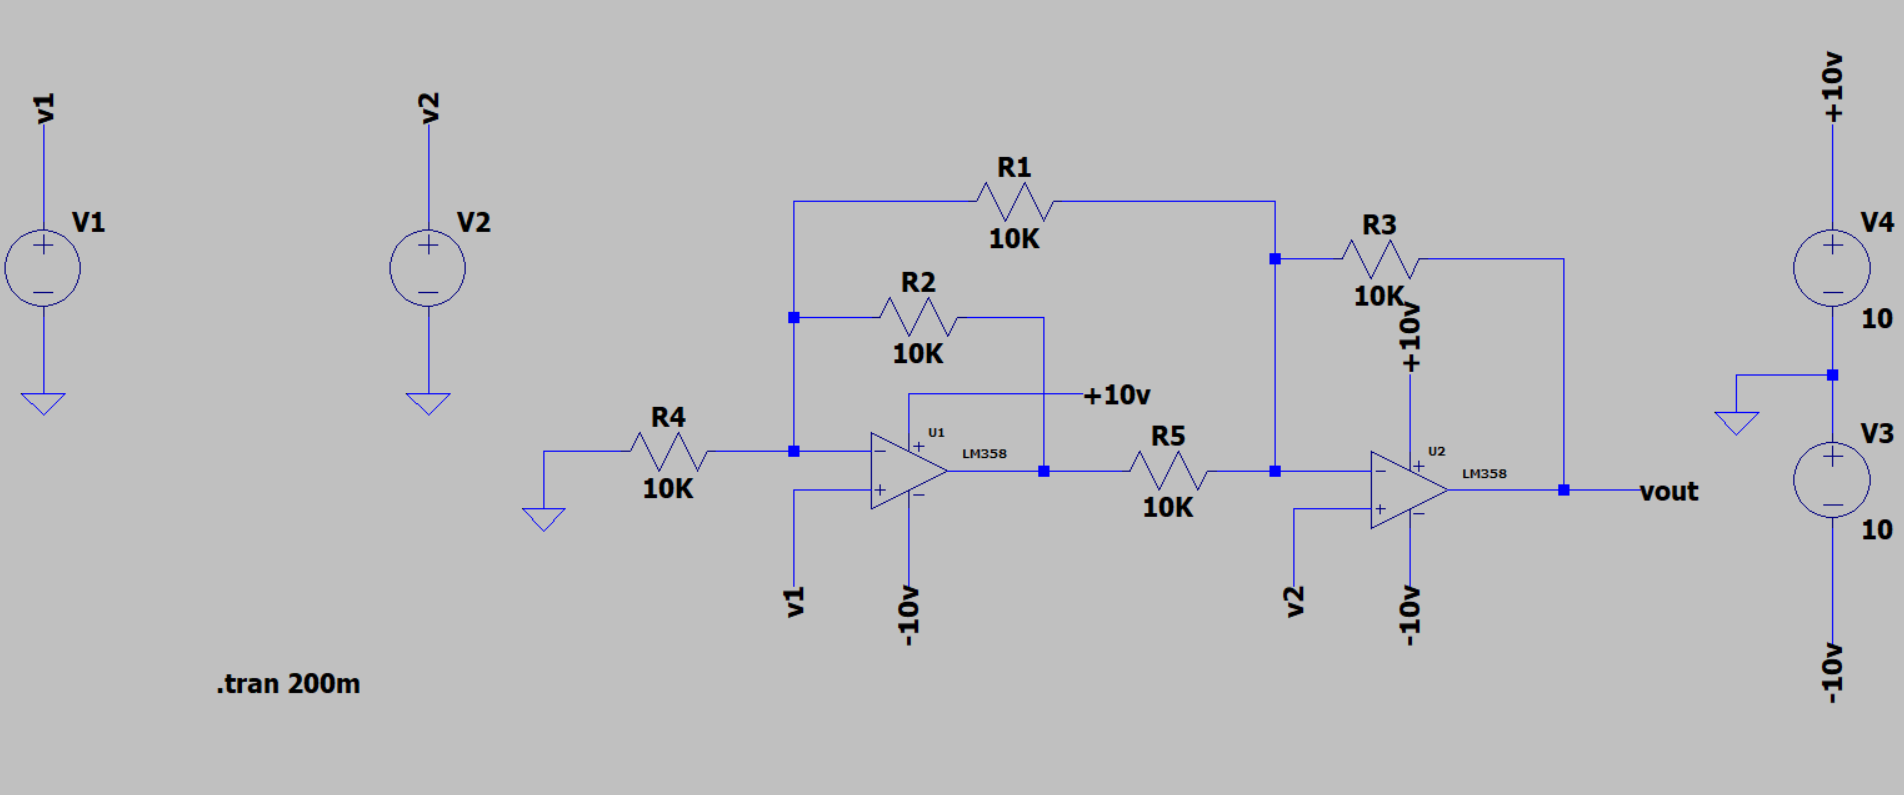
\includegraphics[width=1\linewidth]{Secciones/Circuito1/circuito1_simulacion.png}
    \caption{Señal de salida para modo diferencial - Circuito 1}
    \label{fig:Circuito1Simulacion}
\end{figure}

\hspace{1mm} Se tiene con señal de entrada en modo diferencial:

\begin{figure}[h!]
    \centering
    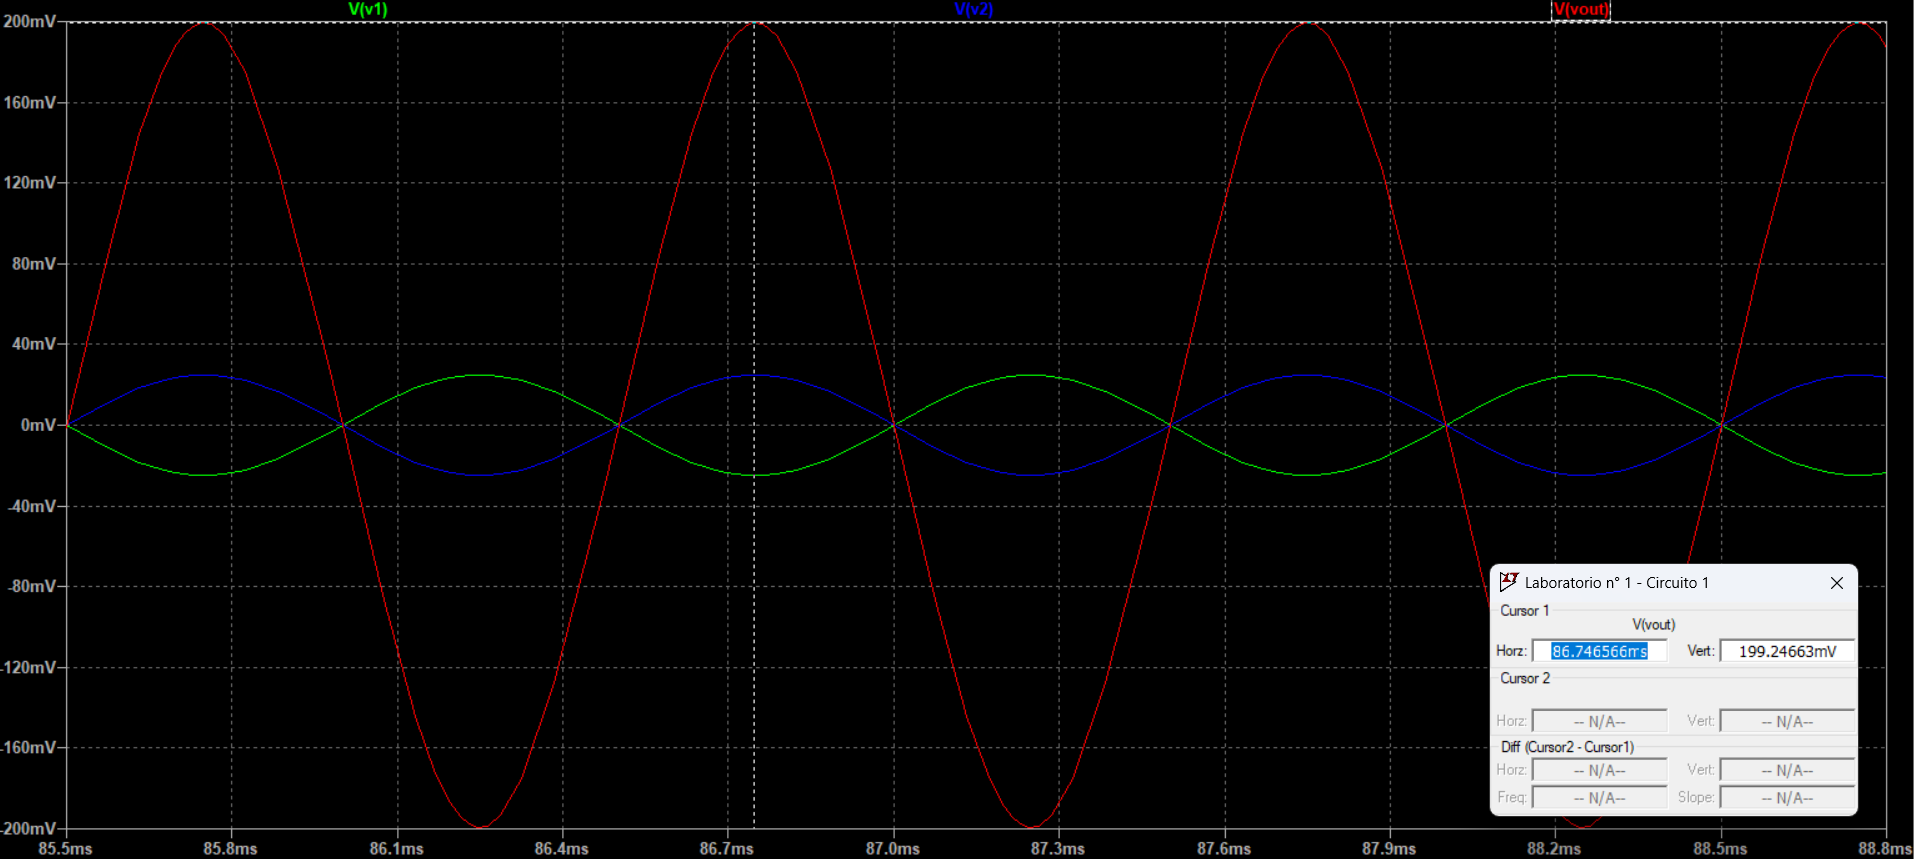
\includegraphics[width=1\linewidth]{Secciones/Circuito1/circuito1_diferencial.png}
    
    \caption{Señal de salida para modo diferencial - Circuito 1}
    \label{fig:Circuito1Diferencial}
\end{figure}

Se realizan las siguientes mediciones:

%   QUITO ESTA FIGURA
% \begin{figure}[h!]
%     \centering
%     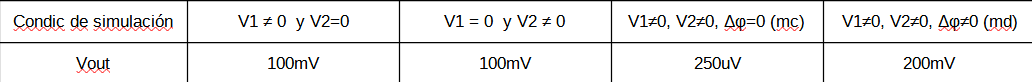
\includegraphics[width=1\linewidth]{Secciones/Circuito1/tabla mediciones.png}
    
%     \caption{Tabla de mediciones}
%     \label{fig:enter-label}
% \end{figure}

%   REEMPLAZO FIGURA ANTERIOR CON ESTA TABLA
\begin{table}[H]
\centering
\begin{tabular}{ | m{2cm} | m{2cm}| m{2cm} | m{2cm} | m{2cm} | } 
  \hline
  Condic. de simulación & $V1 \neq 0$ y $V2 = 0$ & $V1 = 0$ y $V2 \neq 0$ & $V_c \neq 0$ & $V_d \neq 0$ \\ 
  \hline
  $V_{out}$ & 100 mV & 100 mV & 250 uV & 200 mV \\ 
  \hline
\end{tabular}
\caption{Mediciones del circuito}
\end{table}

Se realizan barridos de tensión continua desde -10V a 10V para las fuentes \(v_1\) y \(v_2\). Se grafican las salidas de las dos etapas que conforman el circuito propuesto.

\subsubsection{Barrido para v1}

\begin{figure}[h!]
    \centering
    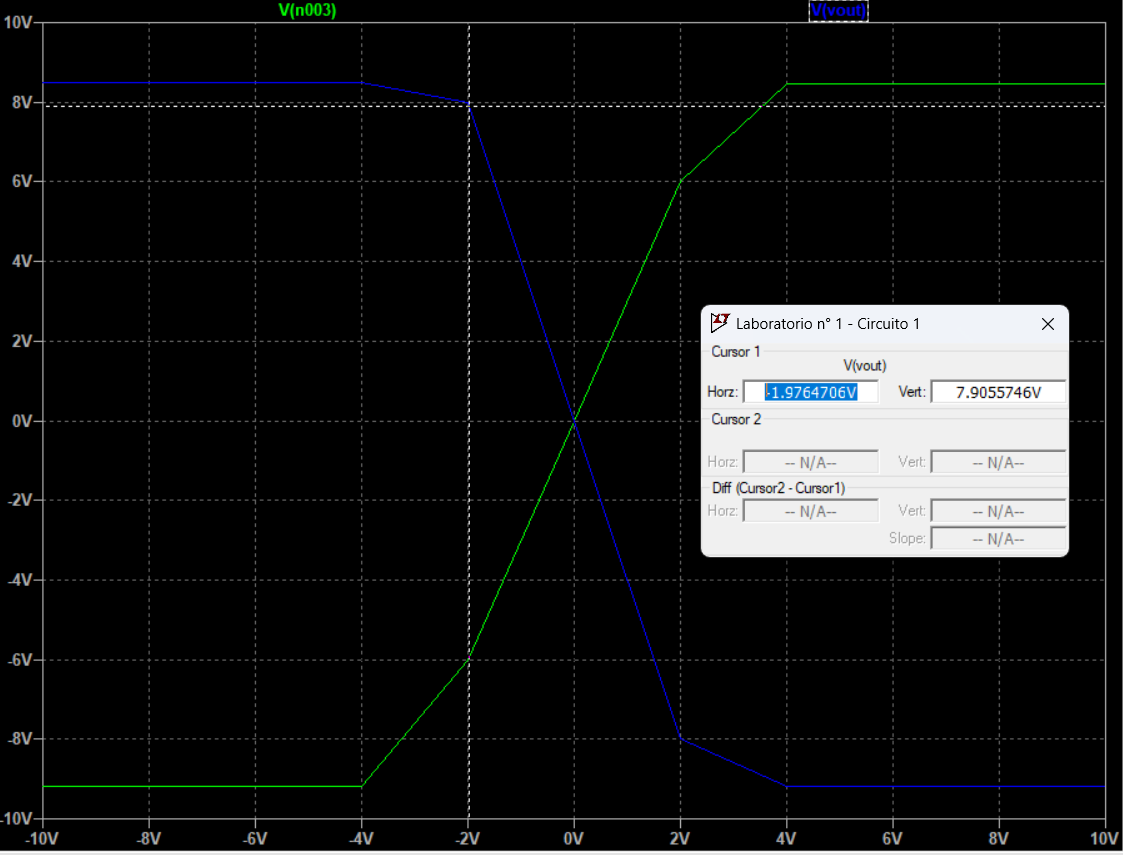
\includegraphics[width=0.7\linewidth]{Secciones/Circuito1/Barrido1.png}
    
    \caption{Barrido en DC para v1}
\end{figure}

Se observa que para baja excursión, las salidas son las rectas \(v_{o1}= 3v1\) y \(v_{o2}= -4v1\), anteriormente analizadas.

\subsubsection{Barrido para v2}
\begin{figure}[h!]
    \centering
    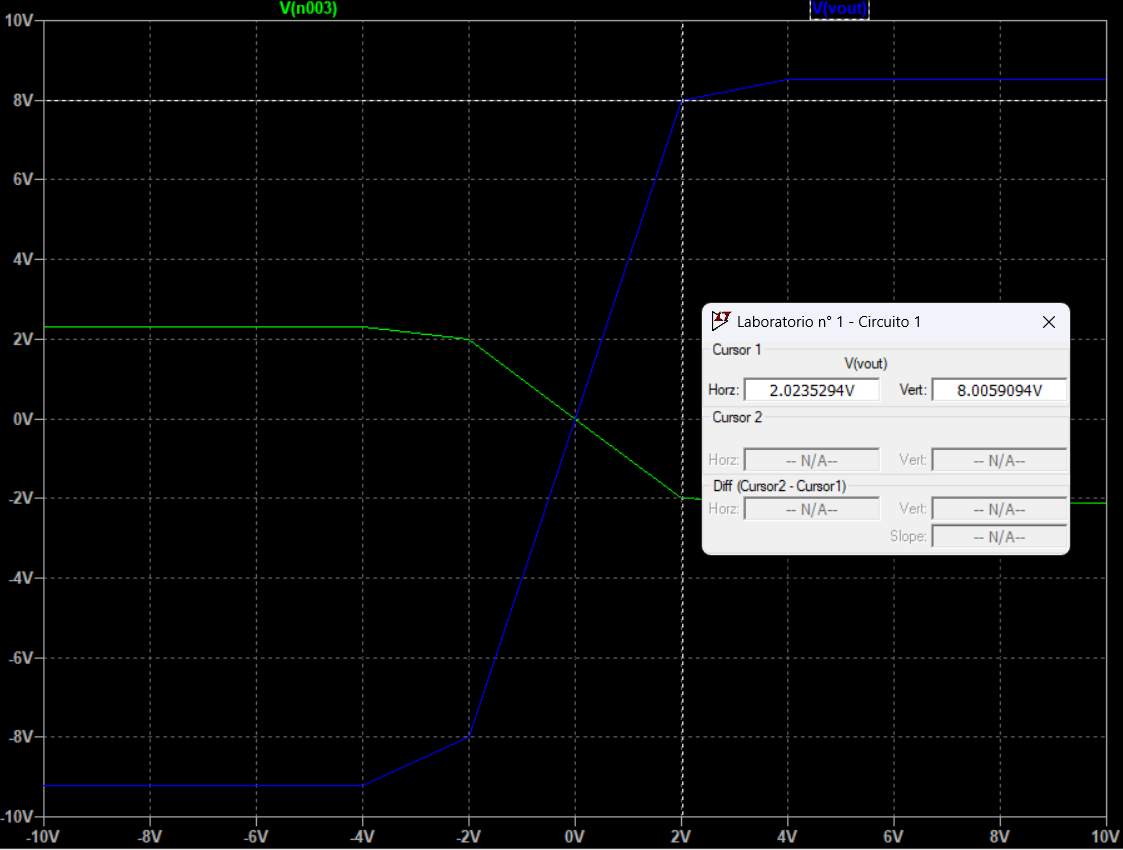
\includegraphics[width=0.7\linewidth]{Secciones/Circuito1/Barrido2.png}
    
    \caption{Barrido en DC para v2}
\end{figure}
Se observa que para baja excursión, las salidas son las rectas \(v_{o1}= -v_2\)  y \(v_{o2}= 4v2\).

\subsubsection{Barrido para modo común}

En este caso se inyecta la misma señal a las entradas y se realizza el mismo barrido de -10V a 10V.
\begin{figure}[H]
    \centering
    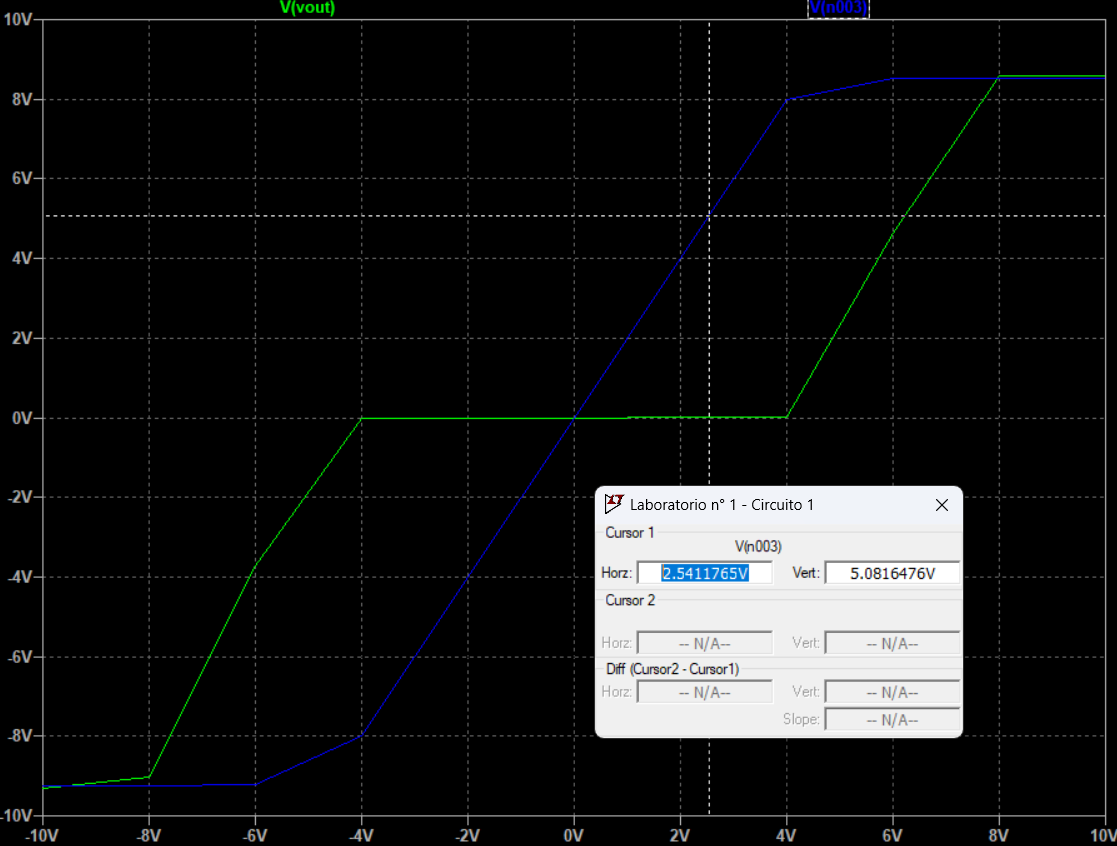
\includegraphics[width=1\linewidth]{Secciones/Circuito1/Barrido mc.png}
    
    \caption{Barrido en DC, modo común}
\end{figure}
Se observa la ausencia de modo común en la salida. Esto ocurre en el rango comprendido entre \(+/-4V\).

